\documentclass[a4paper, 12pt]{article}

% Добавляем новые пакеты
\usepackage[T1, T2A]{fontenc}           % Загружаем пакет с поддержкой кирилицы
\usepackage[utf8]{inputenc}             % Загружаем пакет с поддержкой кодировки файла и символов
\usepackage[english, russian]{babel}    % Пакет для поддержки русского языка
\usepackage{subfig}
\usepackage{graphicx}                   % Загружаем пакет для добавления различной графики (pdf, jpg, png)
\usepackage{import}                     % Загружаем пакет для продвинутого импорта, в частности изображений pdf_tex из графического редактора inkscape (\import{<path to file>}{<filename>.pdf_tex})
\usepackage{subcaption}                 % Пакет для поддержки сетки из фигур, например в две колонки или матрицей
\usepackage{float}                      % Пакет для улучшенного размещения изображенией (ниже используется опция H в команде \begin{figure}[H])
\usepackage{geometry}                   % Пакет для управления отступами на странице (см. далее вызываем \geometry)
\usepackage{amsmath}                    % Добавляем крутую поддержку математики, в частности /align
\usepackage{amsfonts}                   % Пкет с мтематическими шрифтами вроде \mathbb и др.
\usepackage{tabu}                       % Пакет с прокаченными таблицами
\usepackage{booktabs}                   % Крутые вертикальные разделители
\usepackage[dvipsnames]{xcolor}         % Рассширенная поддержка цветов
\usepackage[colorlinks]{hyperref}
\usepackage{indentfirst}                % Пакет, чтобы починить красную строку
\usepackage{listings}                   % Поддержка листингов, оформления кода программы


% Устанавливает отступы на странице
\geometry{left=2cm, right=2cm, bottom=2cm, top=2cm}

% Настараиваем красивые цвета для ссылок на формулы, фигуры (изображения) и другие элементы.
\hypersetup{
    linkcolor=blue,
    filecolor=magenta,
    urlcolor=cyan
}

% Настраиваем супер красивые листинги с попомщью пакетов listings и xcolor
\definecolor{codegreen}{rgb}{0,0.6,0}
\definecolor{codegray}{rgb}{0.5,0.5,0.5}
\definecolor{codepurple}{rgb}{0.58,0,0.82}
\definecolor{backcolour}{rgb}{0.95,0.95,0.92}

\lstdefinestyle{codestyle}{
    backgroundcolor=\color{backcolour},
    commentstyle=\color{codegreen},
    keywordstyle=\color{magenta},
    numberstyle=\tiny\color{codegray},
    stringstyle=\color{codepurple},
    basicstyle=\ttfamily\footnotesize,
    breakatwhitespace=false,
    breaklines=true,
    captionpos=b,
    keepspaces=true,
    numbers=left,
    numbersep=5pt,
    showspaces=false,
    showstringspaces=false,
    showtabs=false,
    tabsize=2
}

\lstset{style=codestyle}
\lstset{extendedchars=\true}

\begin{document}


\section{Фильтрация звука}

В данном задании нам  нужно будет отфильтровать исходный звуковой сигнал. Для начала построим модуль Фурье-образа для него.

\begin{figure}[H]
    \centering
    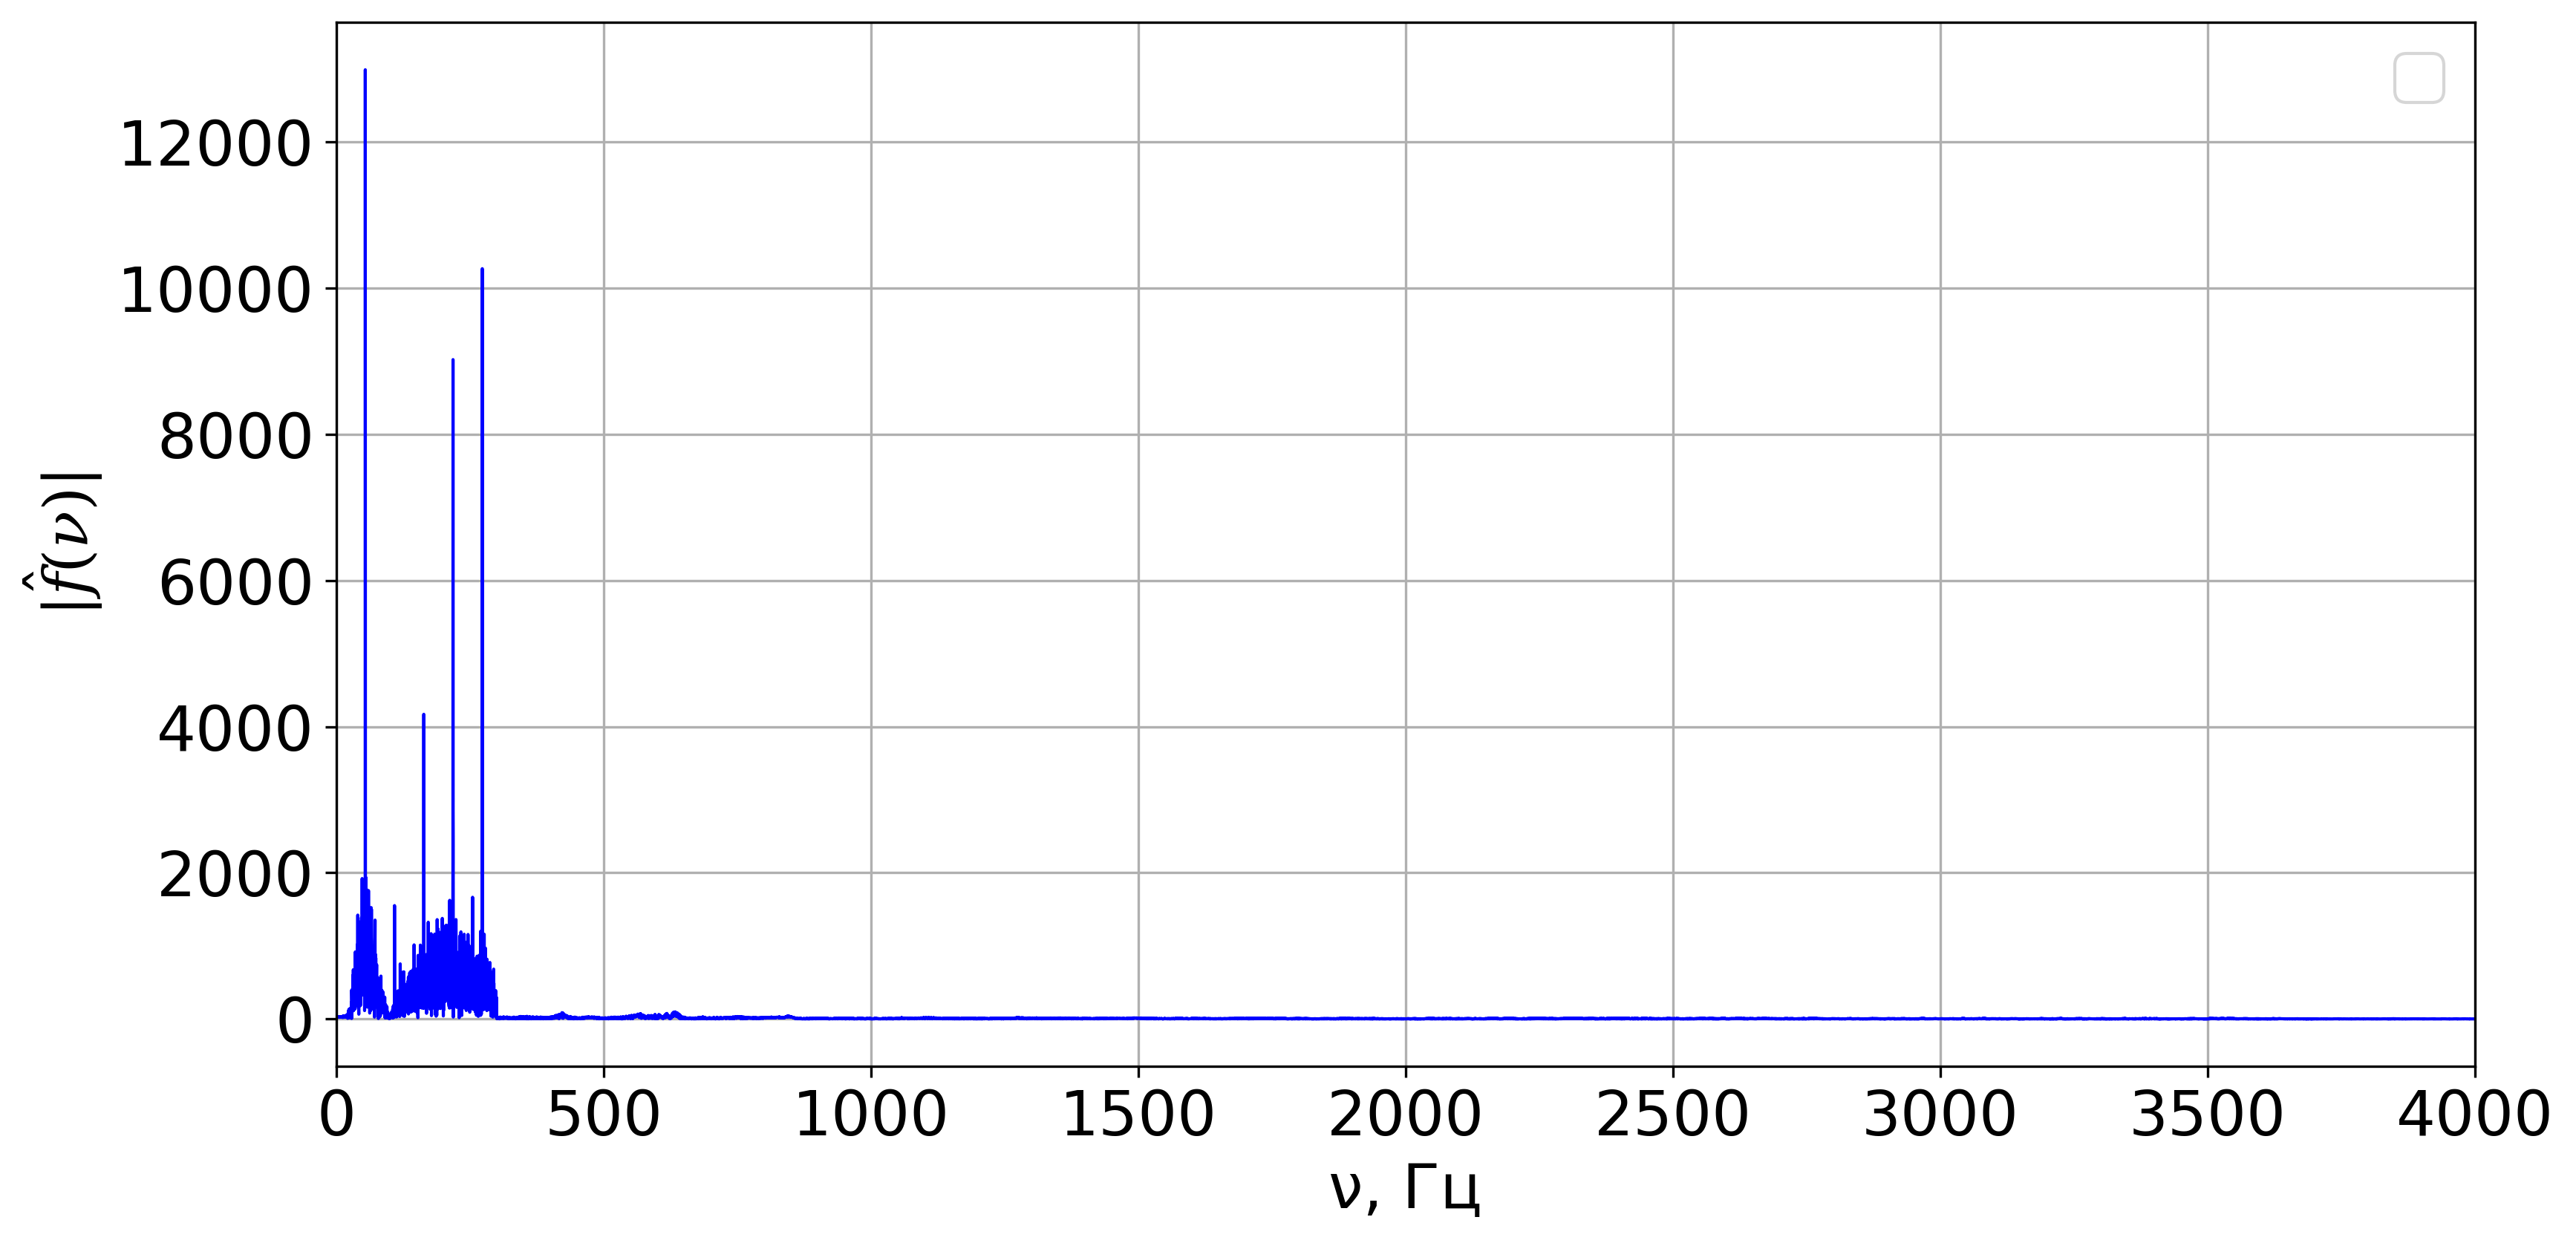
\includegraphics[width=1\linewidth]{figures/fft_original_0_4000.png}
    \caption{График модуля Фурье-образа по частоте исходного сигналав диапазоне 0-4000Гц}
    \label{fig:placeholder}
\end{figure}

\begin{figure}[H]
    \centering
    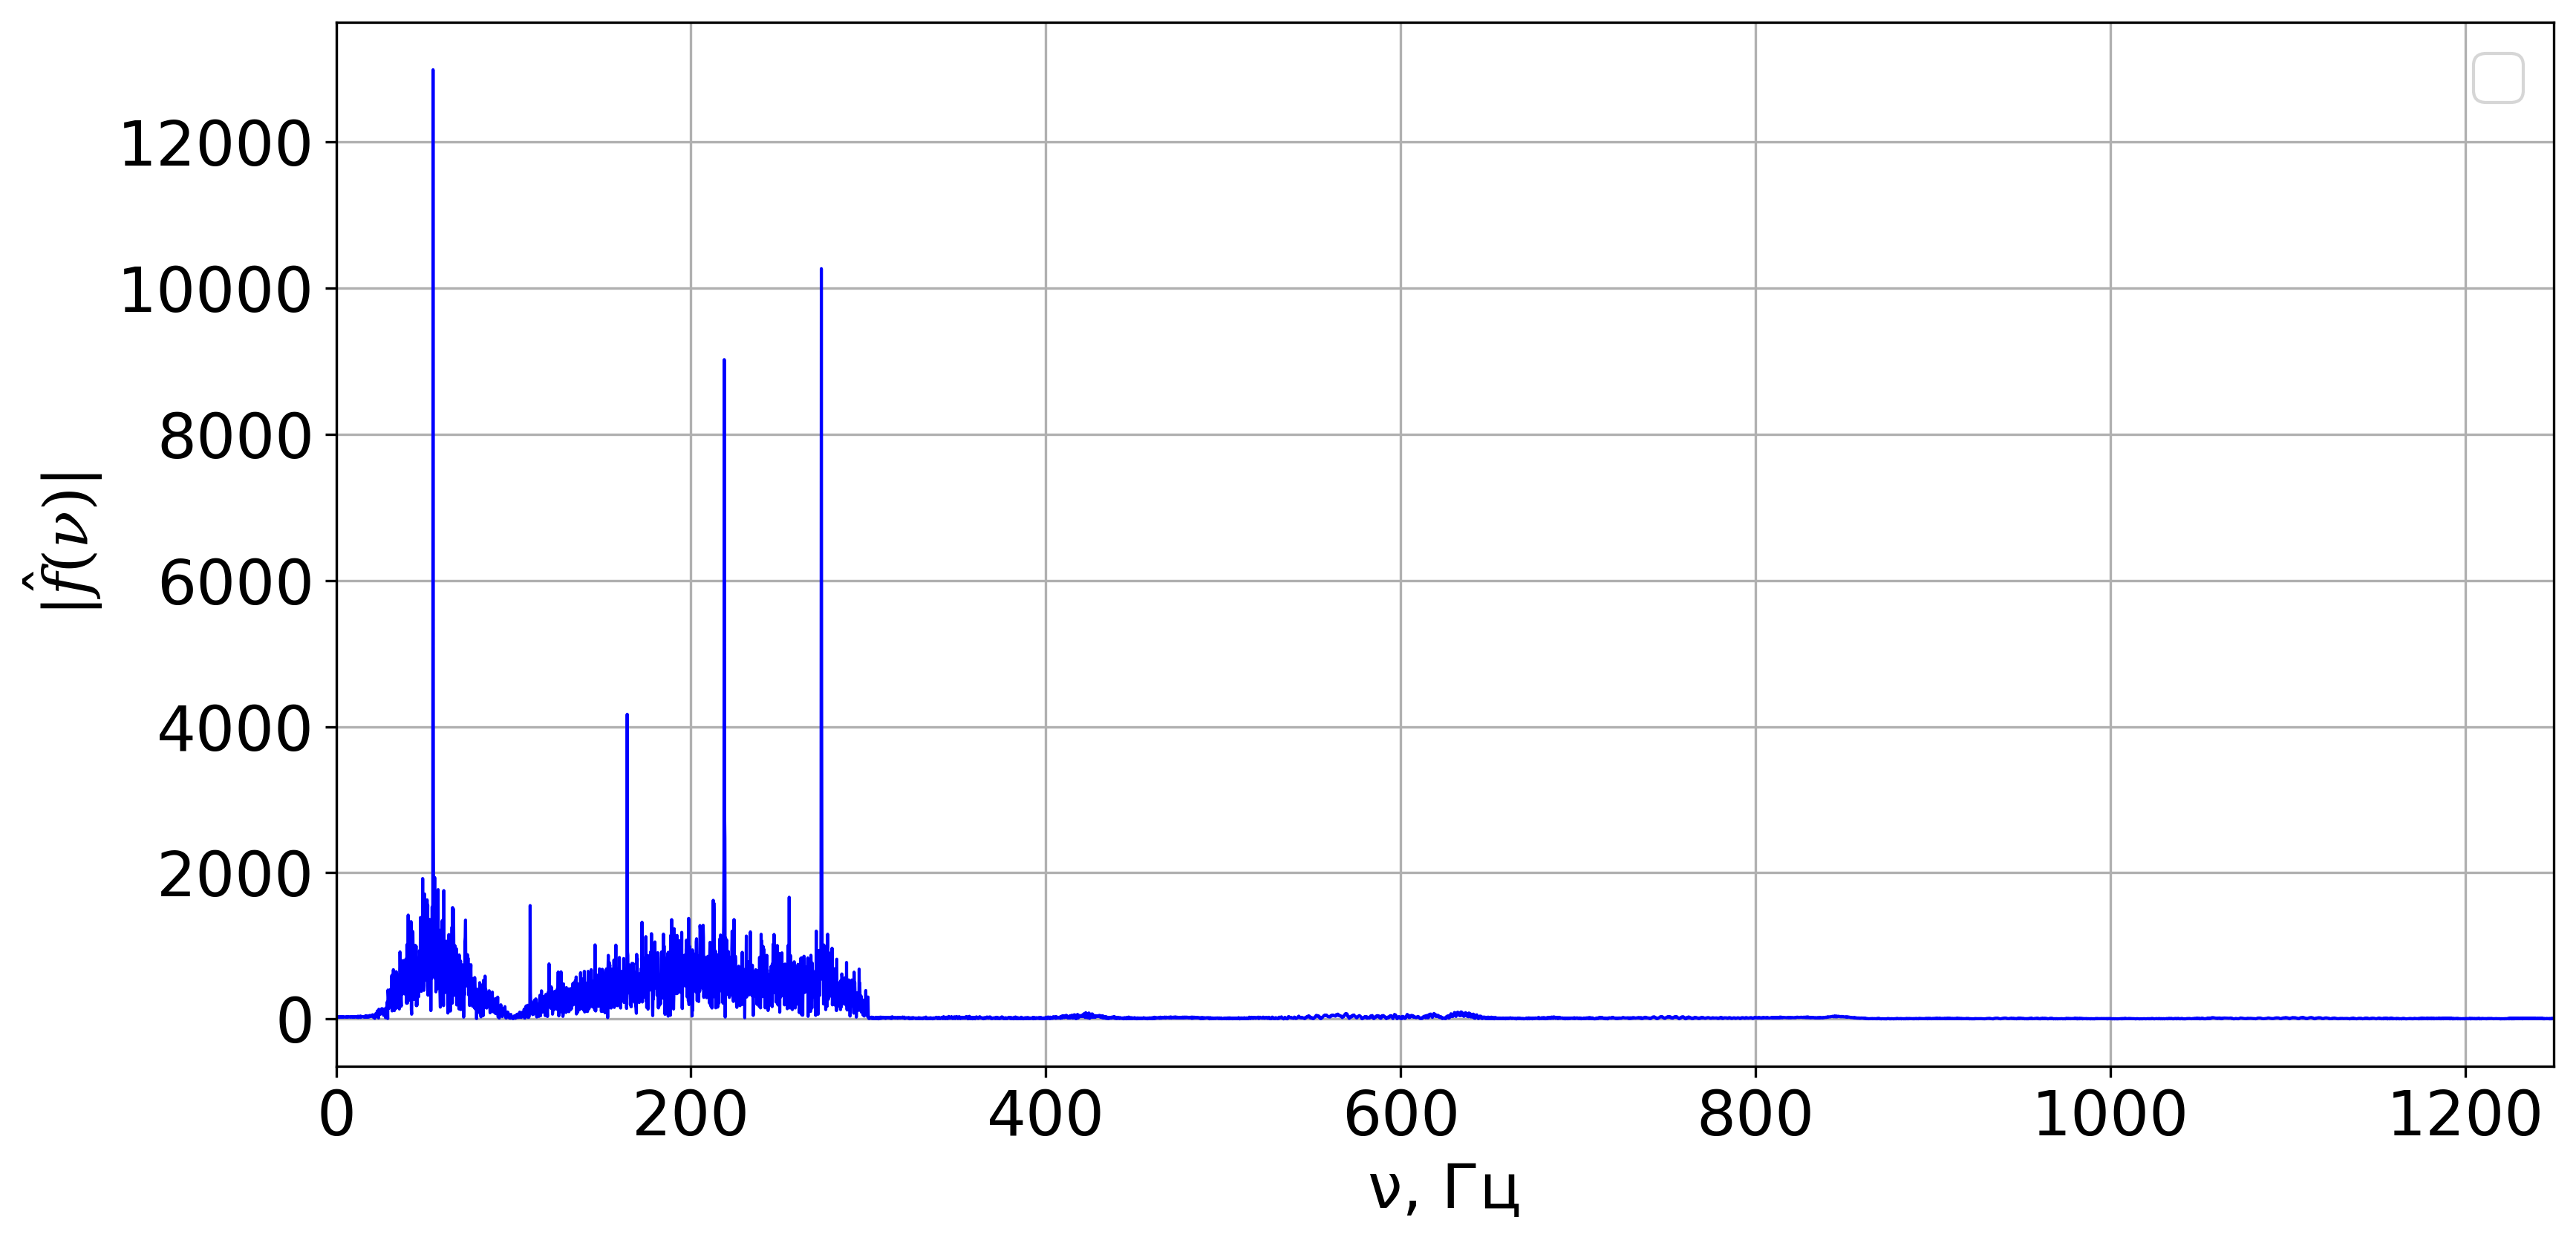
\includegraphics[width=1\linewidth]{figures/fft_original_0_1250.png}
    \caption{График модуля Фурье-образа по частоте исходного сигнала в диапазоне 0-1250Гц}
    \label{fig:placeholder}
\end{figure}

По получившимся графикам можем заметить изобилие шумов в диапазоне 0-300Гц. Выберем диапазон 300–3000 Гц, так как именно в нём сосредоточены основные информативные компоненты речи, обеспечивающие её разборчивость. Применим в этом диапазоне полосовой фильтр, чтобы избавится от шумовых компонент вне речевого диапазона, тогда получим следующий график:

\begin{figure}[H]
    \centering
    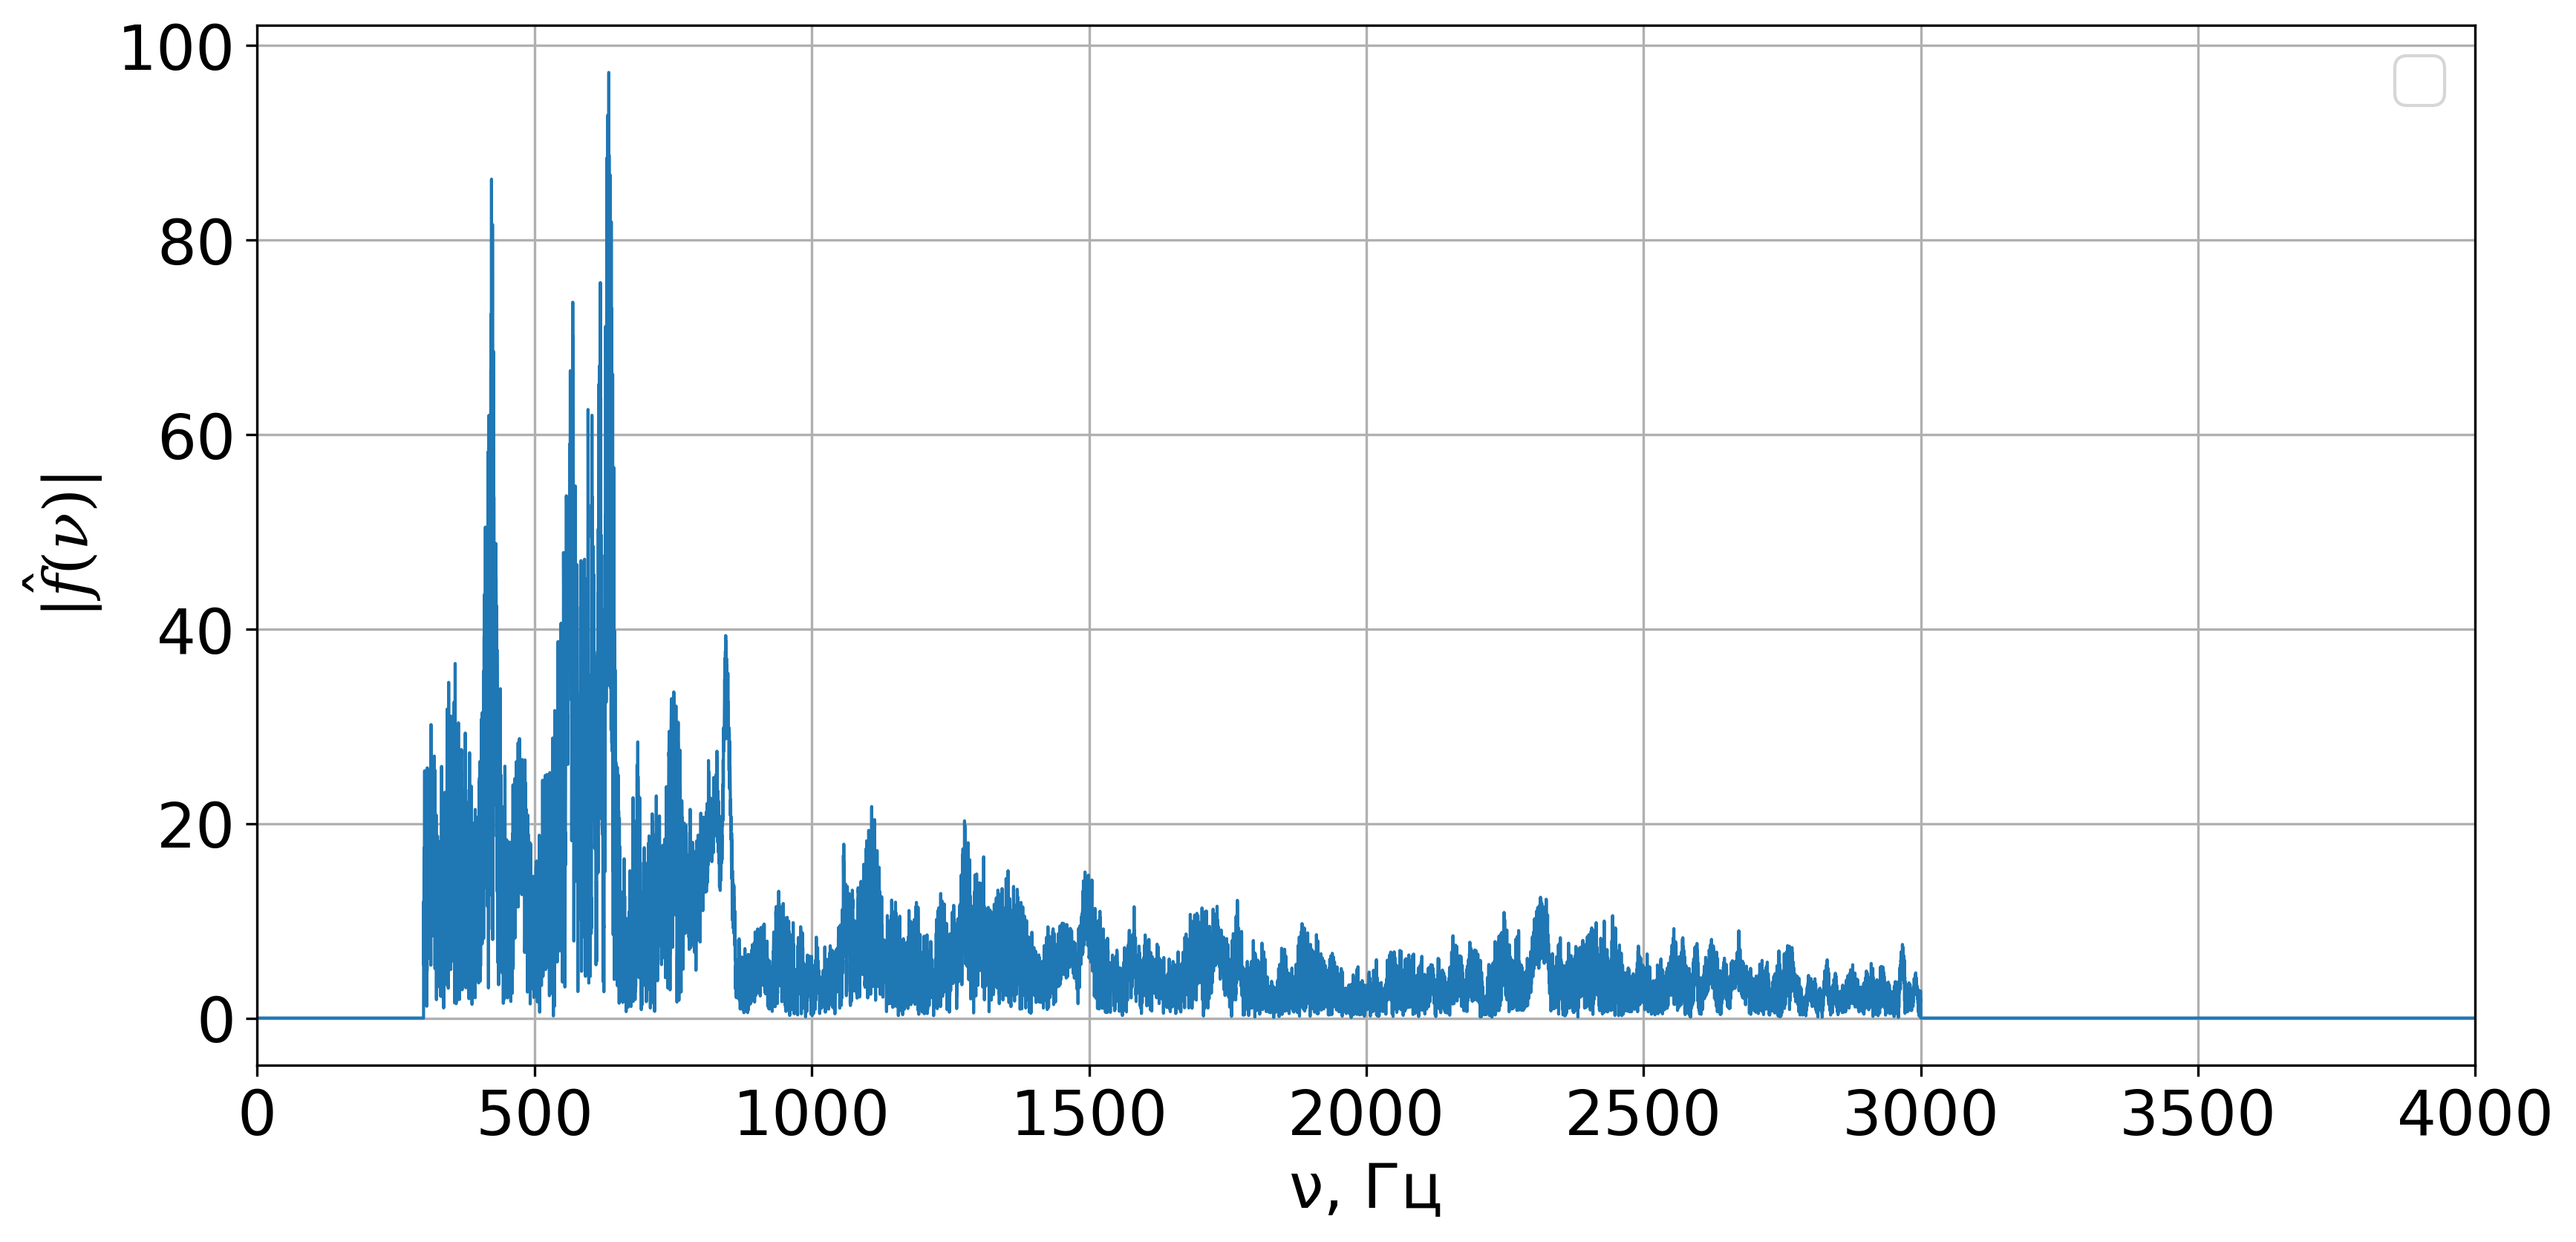
\includegraphics[width=1\linewidth]{figures/fft_filtered_0_4000.png}
    \caption{График модуля Фурье-образа по частоте исходного сигнала в диапазоне 0-1250Гц}
    \label{fig:placeholder}
\end{figure}

После обратного преобразования Фурье к получившемуся образу сравнить графики звуковых сигналов.

\begin{figure}[H]
    \centering
    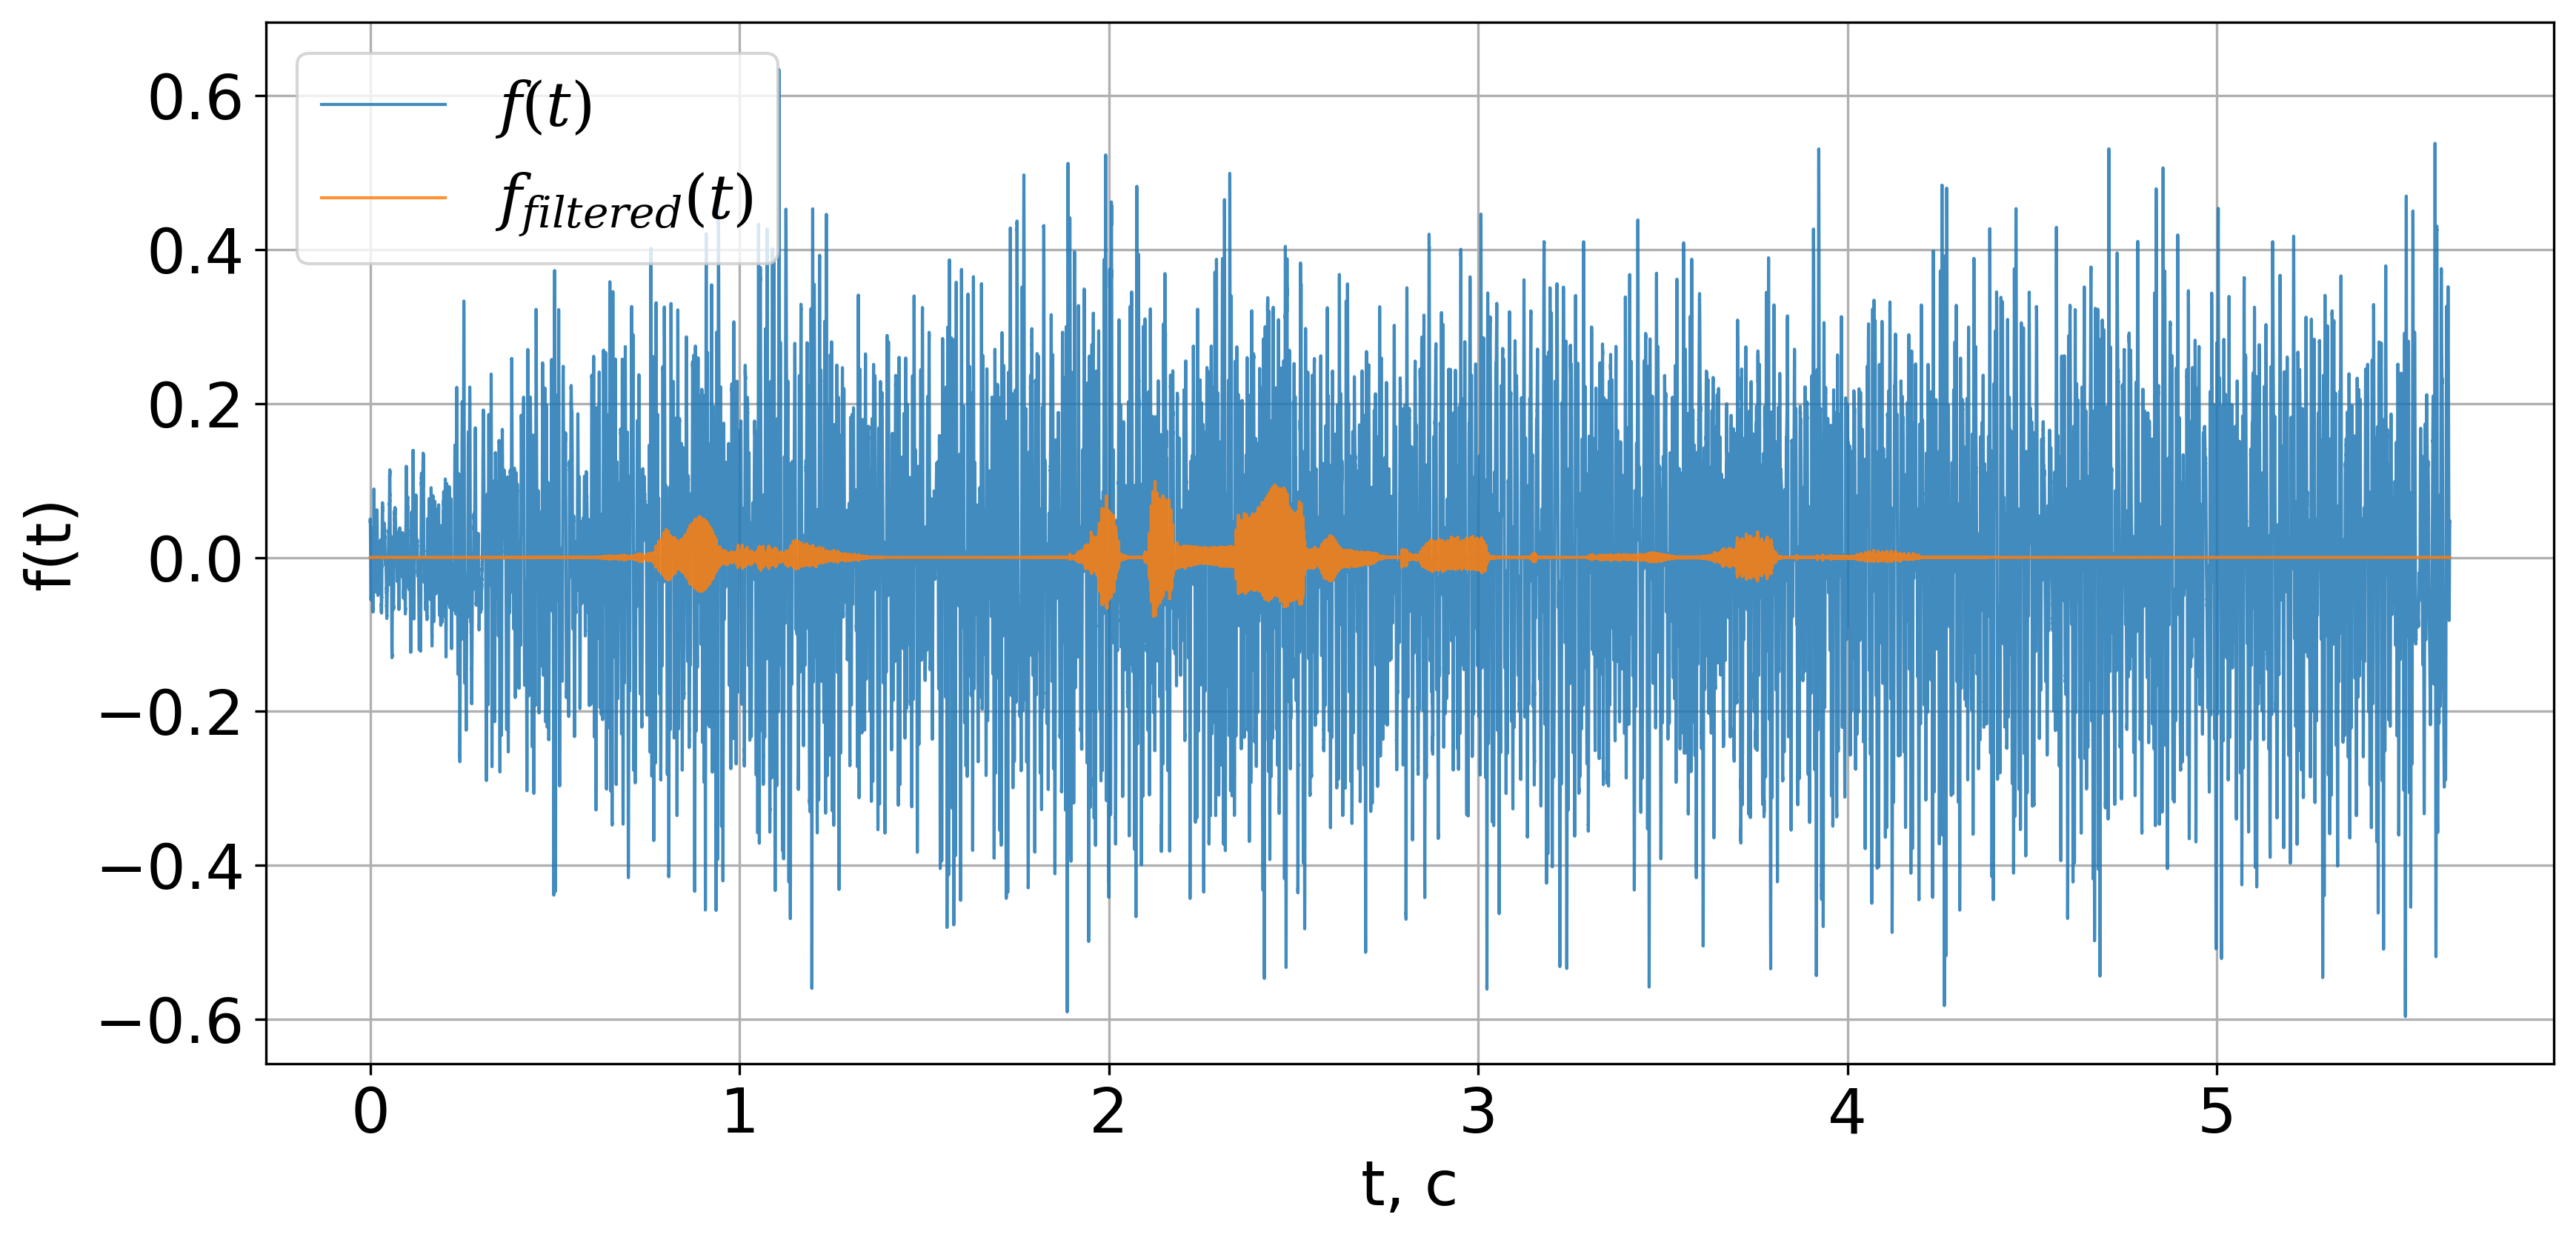
\includegraphics[width=1\linewidth]{figures/time_signals_compare.png}
    \caption{Графики звуковых сигналов}
    \label{fig:placeholder}
\end{figure}

На сравнительном графике заметим, что исходный сигнал содержит колебания на протяжении всей записи,что указывает на наличие дополнительных компонент, не относящихся к полезному сигналу, тогда как в отфильтрованном сигнале заметны только отдельные участки, соответствующие речевому сигналу. Вне этих участков сигнал близок к нулю, что указывает на подавление нежелательных компонент и выделение полезной части сигнала.

После фильтрации в звуковой записи появились артефакты, их появление связано с применением жёсткого полосового фильтра, который резко ограничивает спектр сигнала. В результате чего могут становиться более заметными узкие высокочастотные компоненты и возникать артефакты, обусловленные резким отсечением частот.

\medskip

\textbf{Вывод:}

Выбранный полосовой фильтр подавил шумы, оставив только голос, что подтверждает сравнение графиков звуковых сигналов, и небольшое количество артефактов, появление которых связано с типом фильтрации. Таким образом можно заключить, что жёсткая фильтрация является эффективным способом выделения полезной части сигнала за счёт ограничения его спектра заданным диапазоном частот. При этом резкое обнуление спектральных компонент вне полосы пропускания может приводить к искажению формы сигнала во временной области и появлению характерных артефактов, что указывает на компромисс между степенью подавления помех и качеством восстановленного сигнала.

\end{document}